\documentclass[11pt,letterpaper]{article}
\usepackage[margin=0.82in]{geometry}
\usepackage{amsmath,amssymb,booktabs,array,graphicx,float,microtype}
\usepackage[colorlinks=true,linkcolor=blue,urlcolor=blue]{hyperref}
\pagestyle{plain}
\setlength{\parindent}{0pt}\setlength{\parskip}{5pt}
\setlength{\emergencystretch}{2em}\setlength{\intextsep}{8pt}
\newcommand{\rNZMean}{0.00694248}
\newcommand{\rJYMean}{0.00531169}
\newcommand{\rNZErr}{-0.00762}
\newcommand{\rJYErr}{0.00876}
\newcommand{\rNZVarErr}{-1.35172}
\newcommand{\rJYVarErr}{1.32057}
\newcommand{\rOptRate}{7.84687}
\newcommand{\rOptPeriods}{9.17563}
\newcommand{\rQ}{1.59205}
\newcommand{\rDelta}{-0.36193}
\newcommand{\rForeign}{1.57621}
\newcommand{\rFloor}{-6.68361}
\newcommand{\rSlope}{1.57621}
\newcommand{\rPut}{1.94046}
\newcommand{\rCall}{4.18764}
\newcommand{\rUnhedgedDelta}{0.63443}
\newcommand{\rNoHedgeFloor}{-4.24031}
\newcommand{\rJensen}{1.22542}
\newcommand{\rEightTrue}{9.00647}
\newcommand{\rEightCorrectedError}{0.04935}
\newcommand{\rEightRuleError}{-0.07182}
\begin{document}
\begin{center}{\Large\bfseries FINCB9339 Systematic Investment Strategies\\[3pt]
Homework 4: FX Returns, Compounding and Carry}\\[8pt]
Hanyu Zhang (hz3069)\end{center}
\section*{Summary of answers}
\textbf{1(a)--(b): Inverting returns.} If $R$ is an arithmetic return in one quotation,
the opposite quotation returns $R^{inv}=-R/(1+R)$, rather than $-R$ or $1/R$.
Writing $\mu=E[R]$ and $v=\operatorname{Var}(R)$ gives the local approximations
\[
E[R^{inv}]\approx-\frac{\mu}{1+\mu}+\frac{v}{(1+\mu)^3},\qquad
\operatorname{Var}(R^{inv})\approx\frac{v}{(1+\mu)^4}.
\]
The first two moments alone do not determine the exact inverse-return moments.

\textbf{1(c): NZD/JPY data.} The supplied HW3 workbook yields 2,980 daily returns,
January 4, 1999--June 4, 2010. NZD/JPY means JPY per NZD and equals
$(USD/NZD)(JPY/USD)$; JPY/NZD is its reciprocal. Daily sample-distribution means
are \rNZMean{}\% and \rJYMean{}\%, respectively. Applying the formulas in both
directions gives mean errors of \rNZErr{} and \rJYErr{} basis points per day,
and relative variance errors of \rNZVarErr{}\% and \rJYVarErr{}\%.
The approximations are close for this sample, with nonzero higher-moment effects.

\textbf{2(a): Five doubling-time approximations.} With decimal rate $r>0$ and
$L=\ln2$, the exact fractional doubling time is $n=L/\ln(1+r)$.
The five approximations are $L/r$, $0.69/r$, $L(1/r+1/2)$,
$0.69(1/r+1/2)$ and $0.72/r=72/(100r)$.
The $+L/2$ correction improves the small-rate approximation from an $O(1)$ to an
$O(r)$ absolute error. At 8\%, the corrected exact-$L$ formula has relative error
\rEightCorrectedError{}\%, versus \rEightRuleError{}\% for the Rule of 72.

\textbf{2(b): Best rate for the Rule of 72.} Its error is zero at
\textbf{\rOptRate{}\% per period}, where both formulas give
\textbf{\rOptPeriods{} periods}. This is the unique positive-rate intersection.

\textbf{3(a)--(d): Jurek's option overlay.} Set $g=e^{y_J\tau}$, $A=e^{y_I\tau}$,
and let $\delta_p<0$ be the put delta. Eliminating downside spot exposure requires
$q_p=g(1-q_p\delta_p)=g/(1+g\delta_p)$.
Equation (4) is a funded call payoff, so its lower bound is $-q_pAC_t/S_t$.
Above the strike, its slope relative to unhedged carry is
$q_p/g=1/(1+g\delta_p)>1$. Omitting the initial delta hedge sets the hedge
coefficient to zero and gives $q_p=g$, while retaining the put. Only the
zero-strike limit also removes put protection and recovers unhedged carry.
\clearpage
\section{Inverting arithmetic FX returns}
\subsection{Exact reciprocity: answer 1(a)}
Let $S_t>0$ denote units of currency B per unit of currency A. The return to A
measured in B and the reverse return over the identical interval satisfy
\begin{align}
R&=\frac{S_{t+1}}{S_t}-1,\qquad
R^{inv}=\frac{1/S_{t+1}}{1/S_t}-1,\\
(1+R)(1+R^{inv})&=1,\qquad
\boxed{R^{inv}=\frac{1}{1+R}-1=-\frac{R}{1+R}.}
\end{align}
Reciprocity applies to \emph{gross returns}, not net arithmetic returns.
For example, $R=10\%$ implies $R^{inv}=-9.09091\%$, while $R=-10\%$ implies
$R^{inv}=11.11111\%$. Both returns are zero when the exchange rate is unchanged.
In contrast, logarithmic returns are exactly negatives of each other.

The asymmetry has an exact nonnegative component:
\begin{equation}
R+R^{inv}=\frac{R^2}{1+R}\ge0\quad(R>-1).
\end{equation}
Both arithmetic sample means can therefore be positive. This is a consequence of
changing the currency of measurement, rather than an arbitrage or a funded carry profit.
Compounded gross returns over any common multi-period interval remain reciprocal.

\subsection{Moment approximation: answer 1(b)}
Put $h(x)=(1+x)^{-1}-1$ and $\varepsilon=R-\mu$. Since
$h'(\mu)=-(1+\mu)^{-2}$ and $h''(\mu)=2(1+\mu)^{-3}$,
\begin{equation}
h(R)\approx h(\mu)-\frac{\varepsilon}{(1+\mu)^2}
+\frac{\varepsilon^2}{(1+\mu)^3}.
\end{equation}
Taking expectations gives a second-order mean approximation; retaining the linear
random term gives the leading variance approximation:
\begin{align}
\boxed{E[R^{inv}]\approx-\frac{\mu}{1+\mu}+\frac{v}{(1+\mu)^3}},\\
\boxed{\operatorname{Var}(R^{inv})\approx\frac{v}{(1+\mu)^4}}.
\end{align}
Expanding instead around zero gives $E[R^{inv}]\approx-\mu+\mu^2+v$ and
$\operatorname{Var}(R^{inv})\approx v$ at leading order. The centered formulas
retain the exact dependence on $\mu$ and are used in the empirical comparison.

For the quadratic Taylor polynomial, the variance would additionally involve
\begin{equation}
\frac{v}{(1+\mu)^4}-\frac{2\mu_3}{(1+\mu)^5}
+\frac{\mu_4-v^2}{(1+\mu)^6},\qquad
\mu_j=E[(R-\mu)^j].
\end{equation}
The unknown third and fourth moments prevent identification of this expression
from $\mu,v$ alone. It is the polynomial's variance, not a complete higher-order
expansion of the true variance. These are local approximations requiring returns
concentrated away from $-1$. Finite moments of $R$ do not guarantee finite inverse
moments when probability accumulates near $-1$.
\clearpage
\subsection{NZD/JPY and JPY/NZD: answer 1(c)}
The Data sheet of the HW3 Excel workbook contains 2,981 spot observations from
January 1, 1999 to June 4, 2010, with no missing NZD or JPY levels. Its NZD column
is USD per NZD and its JPY column is JPY per USD. Consequently,
\[
S_t^{NZD/JPY}=NZD_t\,JPY_t\quad\text{(JPY per NZD)},\qquad
S_t^{JPY/NZD}=1/(NZD_t\,JPY_t).
\]
Each return uses consecutive supplied dates; the initial date has no return.
All rows, including holidays, are retained. Returns are arithmetic spot returns
and exclude interest accrual, because Question 1 concerns quotation inversion.
Daily means and variances below are unannualized.

For the empirical distribution, $\widehat\mu=N^{-1}\sum R_t$ and
$\widehat v=N^{-1}\sum(R_t-\widehat\mu)^2$, with $N=2,980$.
Using divisor $N$ makes these literal moments of the empirical distribution.
The alternative unbiased sample variance is $N/(N-1)$ times the displayed variance.
\begin{table}[H]\centering\small\setlength{\tabcolsep}{5pt}\caption{Observed daily spot-return moments}
\begin{tabular}{lrrrr}\toprule
Return & Mean (\%) & Variance & Minimum (\%) & Maximum (\%)\\\midrule
NZD/JPY & 0.00694248 & 0.0001218003 & -9.39011 & 10.12767\\
JPY/NZD & 0.00531169 & 0.0001234349 & -9.19630 & 10.36323\\
\bottomrule\end{tabular}\end{table}
\begin{table}[H]\centering\small\setlength{\tabcolsep}{5pt}\caption{Approximations from the opposite quotation. Variance columns show actual and approximate daily variance multiplied by $10^4$; errors equal approximate minus actual.}
\begin{tabular}{lrrrrrr}\toprule
Target & Mean (\%) & Approx. (\%) & Error (bp) & $10^4v$ & $10^4\widehat v$ & Var. error (\%)\\\midrule
JPY/NZD & 0.00531169 & 0.00523549 & -0.00762 & 1.23434936 & 1.21766437 & -1.35172\\
NZD/JPY & 0.00694248 & 0.00703012 & 0.00876 & 1.21800255 & 1.23408713 & 1.32057\\
\bottomrule\end{tabular}\end{table}
\begin{figure}[H]\centering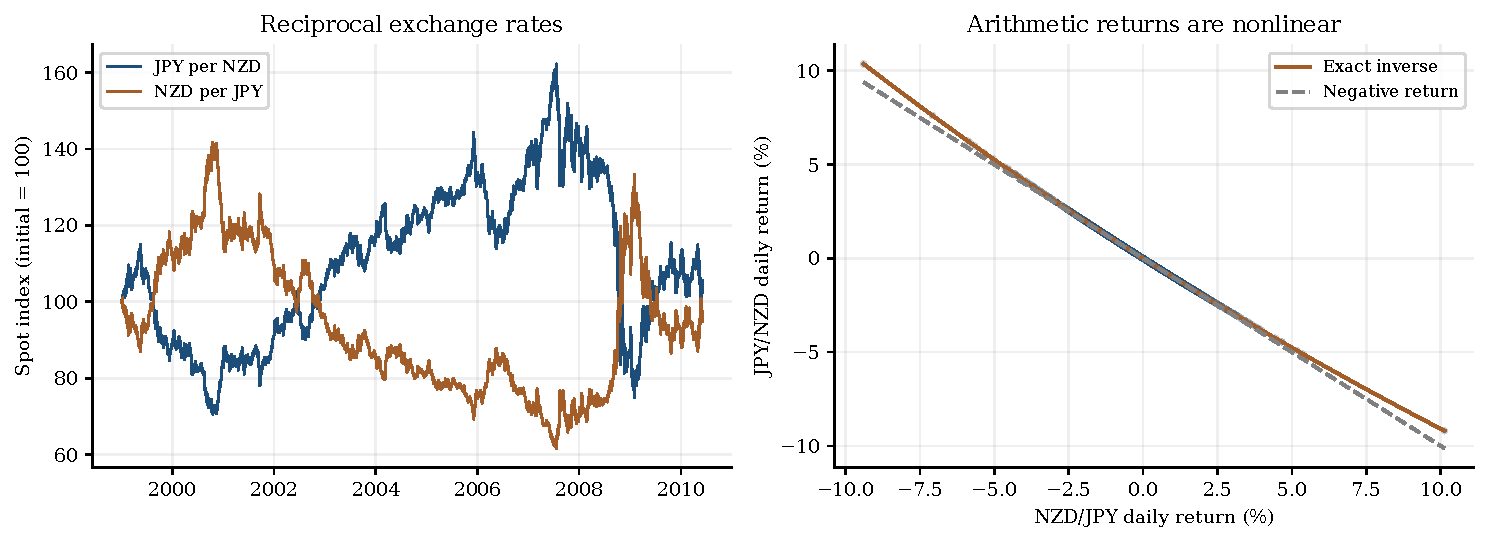
\includegraphics[width=\linewidth,height=2.65in,keepaspectratio]{../results/figures/fx_reciprocity.pdf}\caption{Reciprocal spot indices and the exact nonlinear relationship between arithmetic returns. The dashed line treats inverse returns as negatives and misses the curvature.}\end{figure}

The mean approximation misses the observed inverse mean by less than 0.009 basis
points per day in either direction; the leading variance errors are about 1.3\%.
Thus the data support the approximation's local usefulness, without exact equality.
Negative skew in NZD/JPY increases the importance of large negative observations
under inversion. The exact arithmetic-mean sum is \rJensen{} basis points per day,
consistent with the nonnegative identity above.
\clearpage
\section{Doubling time and the Rule of 72}
\subsection{Exact formula and rate units}
Let $r>0$ be the decimal interest rate per compounding period and let $p=100r$
be its value in percentage points. Discrete compounding implies
\begin{equation}
(1+r)^n=2\quad\Longrightarrow\quad
\boxed{n(r)=\frac{\ln2}{\ln(1+r)}}.
\end{equation}
Thus 8\% corresponds to $r=0.08$, $p=8$, and the Rule of 72 is
$n_{72}=72/p=0.72/r$. This convention resolves the handout's mixed use of a
percentage rate and the factor $100r$ in its denominator. Using $r=8$ in
$72/(100r)$ would give incorrect units and a hundredfold error.

The formula gives a real-valued equivalent number of periods. If growth occurs
only at integer period-end dates, the first doubling occurs at $\lceil n(r)\rceil$.
All approximation errors and the unique intersection below concern the real-valued
$n(r)$. At $r=0$ there is no finite doubling; a constant rate $-1<r<0$ does not double a positive investment.

\subsection{Two approximation families, each with two constants}
Write $L=\ln2=0.693147180559\ldots$. The first family uses
$\ln(1+r)\approx r$, giving $n_0=L/r$. For an improved approximation, invert
the logarithm's small-$r$ expansion:
\begin{align}
\ln(1+r)&=r-\tfrac12r^2+\tfrac13r^3-\cdots,\\
\frac{1}{\ln(1+r)}&=\frac1r+\frac12-\frac{r}{12}+\frac{r^2}{24}+O(r^3),\\
n(r)&=L\left(\frac1r+\frac12\right)-\frac{Lr}{12}+O(r^2).
\end{align}
Retaining $L/r+L/2$ is one order more accurate in absolute error near zero than
$L/r$. With the exact constant, the first formula underestimates $n$ by
$L/2+O(r)$, while the corrected formula overestimates it by $Lr/12+O(r^2)$.
\begin{table}[H]\centering\small\setlength{\tabcolsep}{5pt}\caption{The five approximations: two families evaluated with exact and approximate log constants, plus the Rule of 72}
\begin{tabular}{lrr}\toprule
Method & Decimal-rate form & Percent-rate form\\\midrule
Linear, exact $L$ & $L/r$ & $100L/p$\\
Linear, $0.69$ & $0.69/r$ & $69/p$\\
Corrected, exact $L$ & $L(1/r+1/2)$ & $100L/p+L/2$\\
Corrected, $0.69$ & $0.69(1/r+1/2)$ & $69/p+0.345$\\
Rule of 72 & $0.72/r$ & $72/p$\\
\bottomrule\end{tabular}\end{table}

Using $0.69$ introduces a separate constant-approximation error. It can partly
cancel a Taylor error at some rates, so the corrected $0.69$ formula is not
uniformly better than every alternative at every rate. The improved asymptotic
order compares the two families using the exact same $L$.
\clearpage
\subsection{Interest-rate sensitivity: answer 2(a)}
Evaluate all five formulas on the same 4,991-point grid from 0.1\% to 50\% per
period, spaced by 0.01 percentage points. Define signed absolute error
$e=\widehat n-n$ in periods and signed relative error $100(\widehat n/n-1)$
in percent. The table gives representative doubling times; the plot shows all
five error curves. The period may be a year, month or another fixed interval,
provided the rate and doubling time use the same period.
\begin{table}[H]\centering\small\setlength{\tabcolsep}{5pt}\caption{Doubling times in periods}
\begin{tabular}{lrrrrrr}\toprule
Rate (\%) & Exact & $L/r$ & $0.69/r$ & $L(1/r+.5)$ & $0.69(1/r+.5)$ & $0.72/r$\\\midrule
1.00 & 69.66072 & 69.31472 & 69.00000 & 69.66129 & 69.34500 & 72.00000\\
2.00 & 35.00279 & 34.65736 & 34.50000 & 35.00393 & 34.84500 & 36.00000\\
4.00 & 17.67299 & 17.32868 & 17.25000 & 17.67525 & 17.59500 & 18.00000\\
6.00 & 11.89566 & 11.55245 & 11.50000 & 11.89903 & 11.84500 & 12.00000\\
8.00 & 9.00647 & 8.66434 & 8.62500 & 9.01091 & 8.97000 & 9.00000\\
10.00 & 7.27254 & 6.93147 & 6.90000 & 7.27805 & 7.24500 & 7.20000\\
12.00 & 6.11626 & 5.77623 & 5.75000 & 6.12280 & 6.09500 & 6.00000\\
20.00 & 3.80178 & 3.46574 & 3.45000 & 3.81231 & 3.79500 & 3.60000\\
50.00 & 1.70951 & 1.38629 & 1.38000 & 1.73287 & 1.72500 & 1.44000\\
\bottomrule\end{tabular}\end{table}
\begin{figure}[H]\centering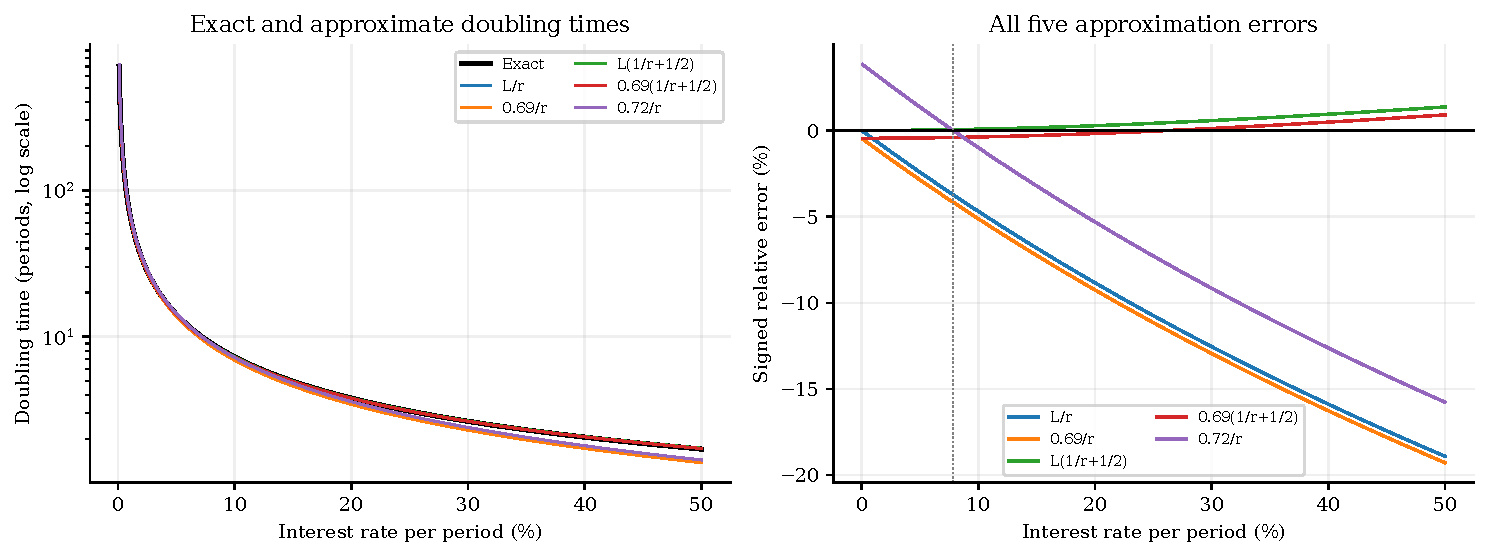
\includegraphics[width=\linewidth,height=3.15in,keepaspectratio]{../results/figures/doubling_sensitivity.pdf}\caption{Exact and approximate doubling times and signed relative errors. $L=\ln2$. The vertical dotted line marks the Rule of 72 intersection; the time axis on the left is logarithmic.}\end{figure}

The exact-$L$ linear formula always underestimates doubling time because
$\ln(1+r)<r$. The $+L/2$ correction removes its leading absolute error and stays
much closer over ordinary rates. The Rule of 72 overestimates at low rates,
crosses the exact value near 7.85\%, and underestimates thereafter. Near zero,
its relative error tends to $100(0.72/L-1)=3.87404\%$; a small rate does not make
that constant error disappear.
\clearpage
\subsection{Error magnitudes and the best Rule of 72 rate: answer 2(b)}
The following maximum absolute relative errors summarize the same grid over
two rate ranges. They measure approximation accuracy, not empirical investment performance.
\begin{table}[H]\centering\small\setlength{\tabcolsep}{5pt}\caption{Maximum absolute relative error (percent)}
\begin{tabular}{lrr}\toprule
Method & 0.1--20\% rates & 0.1--50\% rates\\\midrule
Linear, exact $L$ & 8.83922 & 18.90698\\
Linear, $0.69$ & 9.25313 & 19.27517\\
Corrected, exact $L$ & 0.27686 & 1.36628\\
Corrected, $0.69$ & 0.45403 & 0.90603\\
Rule of 72 & 5.30761 & 15.76540\\
\bottomrule\end{tabular}\end{table}

At 8\%, the exact doubling time is \rEightTrue{} periods, while $n_{72}=9.00000$.
The corrected exact-$L$ expression is $9.01091$ periods, with relative error
\rEightCorrectedError{}\%. This illustrates why the Rule of 72 is particularly
convenient around 8\%, but is not the most accurate general approximation.

Because an exact positive intersection is attainable, both absolute and relative
Rule of 72 errors are minimized to zero there. Equating the two expressions gives
\begin{align}
\frac{0.72}{r_*}&=\frac{L}{\ln(1+r_*)},\\
\frac{\ln(1+r_*)}{r_*}&=\frac{L}{0.72},\\
r_*&=\boxed{0.078468714530153\ldots},\qquad p_* = \rOptRate{}\%.
\end{align}
At this rate, $n_*=\rOptPeriods{}$ periods. The integer number of completed
periods needed to reach at least twice the starting amount is ten.

For uniqueness, define $f(r)=\ln(1+r)/r$ on $r>0$. Then
\begin{equation}
f'(r)=\frac{r/(1+r)-\ln(1+r)}{r^2}<0,
\end{equation}
since $\ln(1+r)>r/(1+r)$. Also $f(0+)=1$ and $f(\infty)=0$.
Because $0<L/0.72<1$, exactly one positive solution exists. The root at $r=0$
of the cross-multiplied equation is extraneous to the original finite-doubling-time problem.
\clearpage
\section{Jurek's crash-neutral currency carry trade}
\subsection{Portfolio construction and put quantity: answer 3(a)}
Use the notation of Jurek (2014), Section 3.1, p. 332. Currency $J$ is the
higher-yield investment currency and $I$ is the funding currency. Write $S_t$
for units of $I$ per $J$, $S_T=S_{t+\tau}$, $K=K_p$, $P=P_t(K,\tau)$,
$C=C_t(K,\tau)$, $g=e^{y_J\tau}$ and $A=e^{y_I\tau}$.
The put's signed initial spot delta is $\delta_p<0$. Prices $P,C$ are in currency
$I$ per unit of underlying $J$; returns are normalized by the base initial spot
notional $S_t$. Rates are continuous, matching the excerpt.

Per base unit of $J$, buy $q_p$ puts and buy an additional $-q_p\delta_p$ units
of $J$ to offset their negative initial delta. The initial foreign deposit is
$B=1-q_p\delta_p$ units of $J$ and the funding-currency borrowing is
$BS_t+q_pP$. At maturity the deposit contains $gB$ units of $J$. Thus Jurek's
Equation (2) is
\begin{equation}
\widetilde R_T=\frac{gBS_T+q_p(K-S_T)^+-A(BS_t+q_pP)}{S_t}.
\label{eq:funded}
\end{equation}
Below $K$, the derivative with respect to $S_T$ is $(gB-q_p)/S_t$.
Eliminating this downside exposure requires $q_p=gB$, hence
\begin{equation}
q_p=g(1-q_p\delta_p)
\quad\Longrightarrow\quad
\boxed{q_p=\frac{g}{1+g\delta_p}.}\label{eq:q}
\end{equation}
This is Equation (3) in the excerpt. One must insure the \emph{maturity} deposit,
including interest on both the base position and the extra delta-hedging currency.
The denominator must be positive. For an ordinary FX put,
$-g^{-1}<\delta_p<0$ in the nondegenerate case, implying a finite positive $q_p$.
The boundary $1+g\delta_p=0$ has no finite position satisfying this construction.

\subsection{Lower bound: answer 3(b)}
With $q_p=gB$, deposit plus put pays $q_p\max(S_T,K)$.
FX put--call parity is $C-P=S_t/g-K/A$, giving
\begin{align}
A(BS_t+q_pP)&=q_pA(S_t/g+P)=q_pAC+q_pK,\\
\widetilde R_T&=q_p\frac{(S_T-K)^+}{S_t}-q_pA\frac{C}{S_t}
\ \ge\ \boxed{-q_pA\frac{C}{S_t}}.\label{eq:call}
\end{align}
This is Equation (4): a nonnegative call payoff less a fixed financed premium.
Equality holds whenever $S_T\le K$. The floor depends on the initial prices,
strike and position size; it does not imply a nonnegative return or a universal
capital-loss bound. The expression is a normalized funded excess payoff, not
an option premium return or a return on the larger gross borrowed notional.
\clearpage
\subsection{Upside slope: answer 3(c)}
For $S_T>K$, Equation~\ref{eq:call} has slope $q_p/S_t$.
Unhedged carry has $R_T^{u}=gS_T/S_t-A$ and slope $g/S_t$. Therefore
\begin{equation}
\boxed{\frac{\partial\widetilde R_T/\partial S_T}
{\partial R_T^{u}/\partial S_T}
=\frac{q_p}{g}=\frac{1}{1+g\delta_p}>1.}
\end{equation}
The additional foreign currency offsets the put's negative initial delta and adds
terminal upside. Initially $B+q_p\delta_p=1$, matching base carry exposure.
This initial match is compatible with a steeper terminal slope: option delta
changes with the exchange rate and time to maturity.

\subsection{Omitting the delta hedge and taking the strike to zero: answer 3(d)}
Omitting the delta hedge sets the \emph{hedging coefficient} to zero, giving
$B=1$ and $q_p=g$. The put retains its actual negative delta, so total initial
delta is $1+g\delta_p<1$. At finite $K$, the put still costs a premium and
provides protection; its above-strike slope equals unhedged carry's $g/S_t$.

For a strictly positive exchange rate, $K\downarrow0$ implies $P,\delta_p\to0$,
$q_p\to g$ and $C\to S_t/g$. Equation~\ref{eq:call} becomes $gS_T/S_t-A$,
recovering unhedged carry. The two cases share a zero hedge coefficient;
only the zero-strike limit removes the put.
\begin{figure}[H]\centering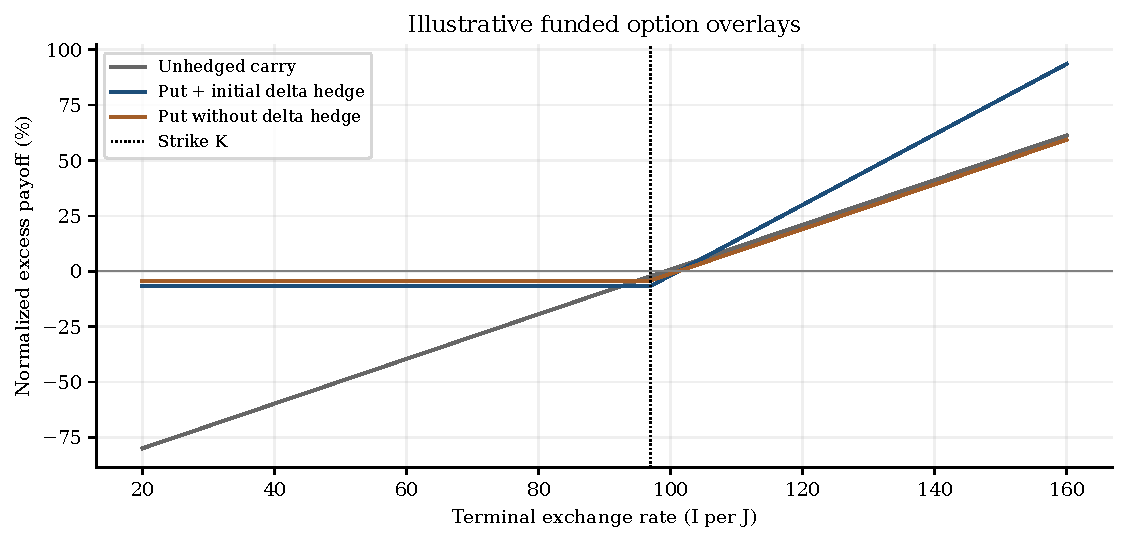
\includegraphics[width=\linewidth,height=2.55in,keepaspectratio]{../results/figures/option_overlay.pdf}\caption{Illustrative funded payoffs, not empirical returns. Continuous annual rates are $y_J=4\%$, $y_I=1\%$, maturity is 0.25 years, $S_t=100$, $K=97$, and FX volatility is 15\%. Option prices use the standard lognormal FX model.}\end{figure}

In this illustration, $P=\rPut{}$, $C=\rCall{}$ and $\delta_p=\rDelta{}$, giving $q_p=\rQ{}$ and $B=\rForeign{}$.
The delta-hedged overlay has slope multiplier \rSlope{} and floor \rFloor{}\%.
Without the delta hedge, the floor is \rNoHedgeFloor{}\% and initial total delta
is \rUnhedgedDelta{}. Delta matching requires a larger position and does not guarantee a higher floor.
Holdings are fixed after initiation and settlement is default-free.

\end{document}
